% Un articolo scritto con LaTeX
\documentclass[a4paper,11pt]{article}
\usepackage{graphicx}
\usepackage[T1]{fontenc} % codifica dei font in uscita
\usepackage[utf8]{inputenc} % lettere accentate da tastiera
\usepackage[italian]{babel} % lingua principale del documento
\usepackage{url}
\usepackage [a4paper, top=2.5cm, bottom=2.5cm, left=1.5cm, right=1.5cm, bindingoffset=8mm] {geometry}

% inizio documento

\usepackage{graphicx}
\begin{document}

\begin{center}
\textbf{\huge Esperienza 1} \\ \vspace{10pt}
\large Alberini Giacomo \\ Bassini Luigi \\ Michele Pedrotti\\ Trevisson Nicola 
\end{center}

\section{Introduzione}
Scopo dell'esperienza è quello di misurare l'andamento della pressione durante la fase di svuotamento di un volume di aria, utilizzando diverse pompe e confrontando i risultati. Successivamente si è cercato di misurare alcune caratteristiche di gas noti e ignoti applicando la legge di stato dei gas ideali. 
\section{Confronto pompe a vuoto}

Inizialmente il gruppo si è preoccupato di misurare il volume del contenitore usato nell'esperienza. Per stimare questa grandezza la bottiglia è stata riempita di acqua e quindi è stato misurato il valore del volume in litri con un cilindro graduato. Il valore ottenuto è il seguente:
$$2.775  ~l\pm 0.009 ~l$$
Il passo successivo consisteva nel creare il vuoto nella camera utilizzando due tipi di pompe: una manuale e l'altra meccanica. \\
Per la prima i risultati sono stati riassunti in un grafico che mostra l'andamento della pressione (misurata con un manometro differenziale al mercurio) al variare del numero di pompaggi manuali effettuati. Con la seconda si è preferito invece sostiuire al numero di pompaggi il tempo misurato in secondi avvalendosi di un cronometro. Sono stati dunque prodotti i due seguenti grafici.

\begin{figure}[htbp]
\centering
\includegraphics[scale=1.00]{grafico_Pt.png}
\label{}
\end{figure}

\begin{figure}[htbp]
\centering
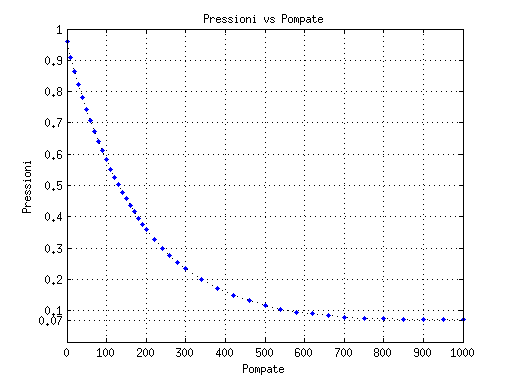
\includegraphics[scale=1.00]{prexpomp.png}
\label{}
\end{figure}

\newpage NOTA: Per la loro ridotta dimensione le barre di errore non risultano visibili all'interno della risoluzione del grafico. Si può anche notare un leggero flesso all'interno del secondo grafico legato alla repentina varizione di pressione che ha procurato un'oscillazione della colonnina di mercurio.\\\\
Come si può notare, entrambi i grafici mostrano un'andamento esponenziale che tende a un valore particolare di pressione, caratteristico dello strumento utilizzato. \\
Il valore limite delle due pompe è apprezzabile dai grafici.\\
Si nota anche che la pompa meccanica (azionata da un motore elettrico) raggiunge un valore di pressione finale minore rispetto a quella manuale.
\\ \\


\textbf{Calcolo della densità dell'aria}

La densità dell'aria a $3 ~atm$ è la seguente $d=3.46 kg/m^3 \pm 0.02$  

\section{Calcolo del peso molare di alcuni gas}
Successivamente si sono calcolati i valori molari di alcuni gas, utilzzando la legge di stato dei gas perfetti. \\Dopo aver calcolato la massa della bottiglia in cui era stato fatto il vuoto utilizzando la pompa meccanica, per differenza sono state calcolate le masse dei diversi gas e quindi, utilizzando la relazione $PV=nRT$ e facendo gli opportuni calcoli, si è giunti ai seguenti risultati: 
\hspace{-140pt}

\begin{center}
\begin{tabular}{|c|c|c|c|c|}
\hline \rule[-2ex]{0pt}{5.5ex} $Gas$ & $Massa [g]$ & $Temperatura [^\circ{C}]$ & $Massa Molare [g/mol]$ & $M. Mol. Tabulato [g/mol]$ \\ 
\hline \rule[-2ex]{0pt}{5.5ex} Elio & $1.3 \pm 0.05$ & $22.7 \pm 0.1$ & $3.9 \pm 0.2$ & 4.002 \\ 
\hline \rule[-2ex]{0pt}{5.5ex} Azoto & $9.2 \pm 0.05$ & $22.4 \pm 0.1$ & $27.9 \pm 0.5$ & 28.034 \\ 
\hline \rule[-2ex]{0pt}{5.5ex} Ignoto & $13.1 \pm 0.05$ & $22.3 \pm 0.1$ & $39.7 \pm 0.7$ & ? \\ 
\hline \rule[-2ex]{0pt}{5.5ex} CO\ped2 & $15.2 \pm 0.05$ & $22.5 \pm 0.1$ & $46.1 \pm 0.8$ & 44.010 \\ 
\hline 
\end{tabular}
\end{center}
\vspace{40pt}

NOTA: nella tabella non sono stati inseriti i volumi, la pressione e il numero di moli perche a valori costanti.\\

Notia